\subsubsection{Design Problems and Solutions}
3D printing is typically an iterative process, where the design is printed, tested, and then modified based on the results.
This further reinforces the need for a modular design, as it allows for easy modification of each component.
After a few iterations with errors due to tolerances and slightly incorrect measurements, (not relevant to the technical content of this report)
I was able to produce a design that physically fit together and mounted the components as intended, however when combined with the software
and electronics, I encountered a few problems that I had to overcome by making some design decisions.

\begin{figure*}
    \begin{minipage}[t]{0.49\textwidth}
        \centering
        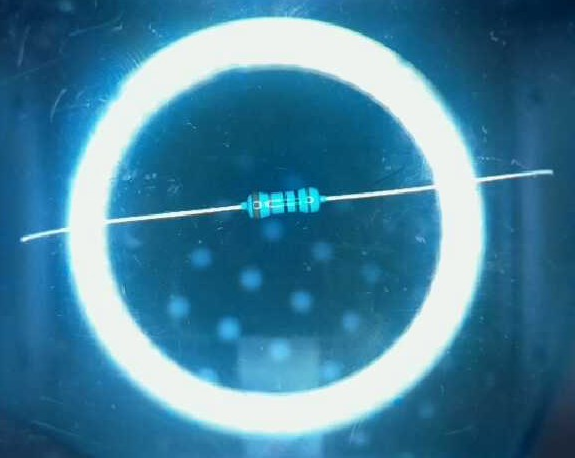
\includegraphics[width=\textwidth]{imgs/design/ringlight.jpg}
        \caption{Glare from LED Ring}
        \label{fig:glare}
    \end{minipage}
    \hfill
    \begin{minipage}[t]{0.49\textwidth}
        \centering
        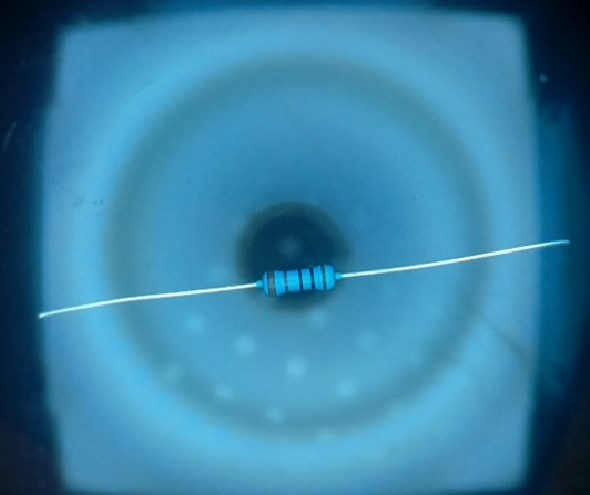
\includegraphics[width=\textwidth]{imgs/design/diffusedlight.jpg}
        \caption{Diffused Light}
        \label{fig:diffusedlight}
    \end{minipage}
\end{figure*}

\noindent
\textbf{Mechanical Design Problems} \\
The first design problem I encountered was the initial design of the LCD display mount. As mentioned in Section \ref*{sec:lcdhousing},
the LCD housing is split into two parts; the LCD cover, where the LCD display slides into, and a base plate, which mounts to the camera housing.
The initial design of the LCD cover only mounted to the base plate using two M3 screws at the bottom Figure \ref*{fig:unbracedscreen}, which made it unstable and prone to wobbling.
Overtime, this would put stress on the plastic, causing it to break. To solve this, I added a third mounting point to the LCD cover in the form of a 
bracket that reaches halfway up the LCD cover, as shown in Figure \ref*{fig:bracedscreen}, increasing the stability of the LCD display preventing it from wobbling.

The second design problem I encountered was the design of the camera housing. As mentioned in Section \ref*{sec:camerahousing}, the camera housing contains the camera and the LED strip.
The camera itself is not a macro lens, but rather a standard lens with an adjustable focus. The workaround is to set the focus as close as possible, and then determine the optimal
distance between the camera and the object to be imaged. This is done by placing an object on the acrylic plate. Initially, the height of the camera housing was too short Figure \ref*{fig:shortcamera}, resulting in a 
blurry image, which was remedied by simply changing the parametric parameters that define the height of the camera housing Figure \ref*{fig:tallcamera}. 
The above design problems were solved by simply modifying the design, however the third design problem was more complex. As mentioned in Section \ref*{sec:camerahousing}, the approach 
to imaging components is to place them on the acrylic plate, and then image them using the camera. However, when doing so, the light from the LED Ring would reflect off the acrylic plate Figure \ref*{fig:glare},
resulting in a incredible glare that would obscure the image of the component. There was an attempt to 3D print a light diffuser to reduce the glare Figure \ref*{fig:diffusedlight}, however this was not effective, and instead
causes the entire image to be affected by the reflection of the LED Ring. This was a major design problem as, in the non-diffused image, any components in the glare of the ring are obscured, and in the diffused image,
the entire image has incorrect colours and is partially obscured. To solve this, three solutions were considered:
\begin{mylist}
  \item \textbf{Polarising Filter} \\
  Polarising filters can be used to reduce glare by filtering out light that is polarised in a certain direction.
  \item \textbf{Different Light Source} \\
  The LED Ring was chosen as it provides a uniform light source as it would surround the camera, however it is possible to use a different light source that does not cause glare, for example
  an LED strip that is mounted above the camera.
  \item \textbf{Down-facing Camera} \\
  Instead of imaging the components from above, the camera can be mounted below the acrylic plate, and the components can be imaged from below.
  The issue is that the light of the LED Ring bounces off the bottom layer of the acrylic plate, so any components on top are obscured.
\end{mylist}
  
\begin{figure*}[t]
  \begin{minipage}[t]{0.24\textwidth}
    \centering
    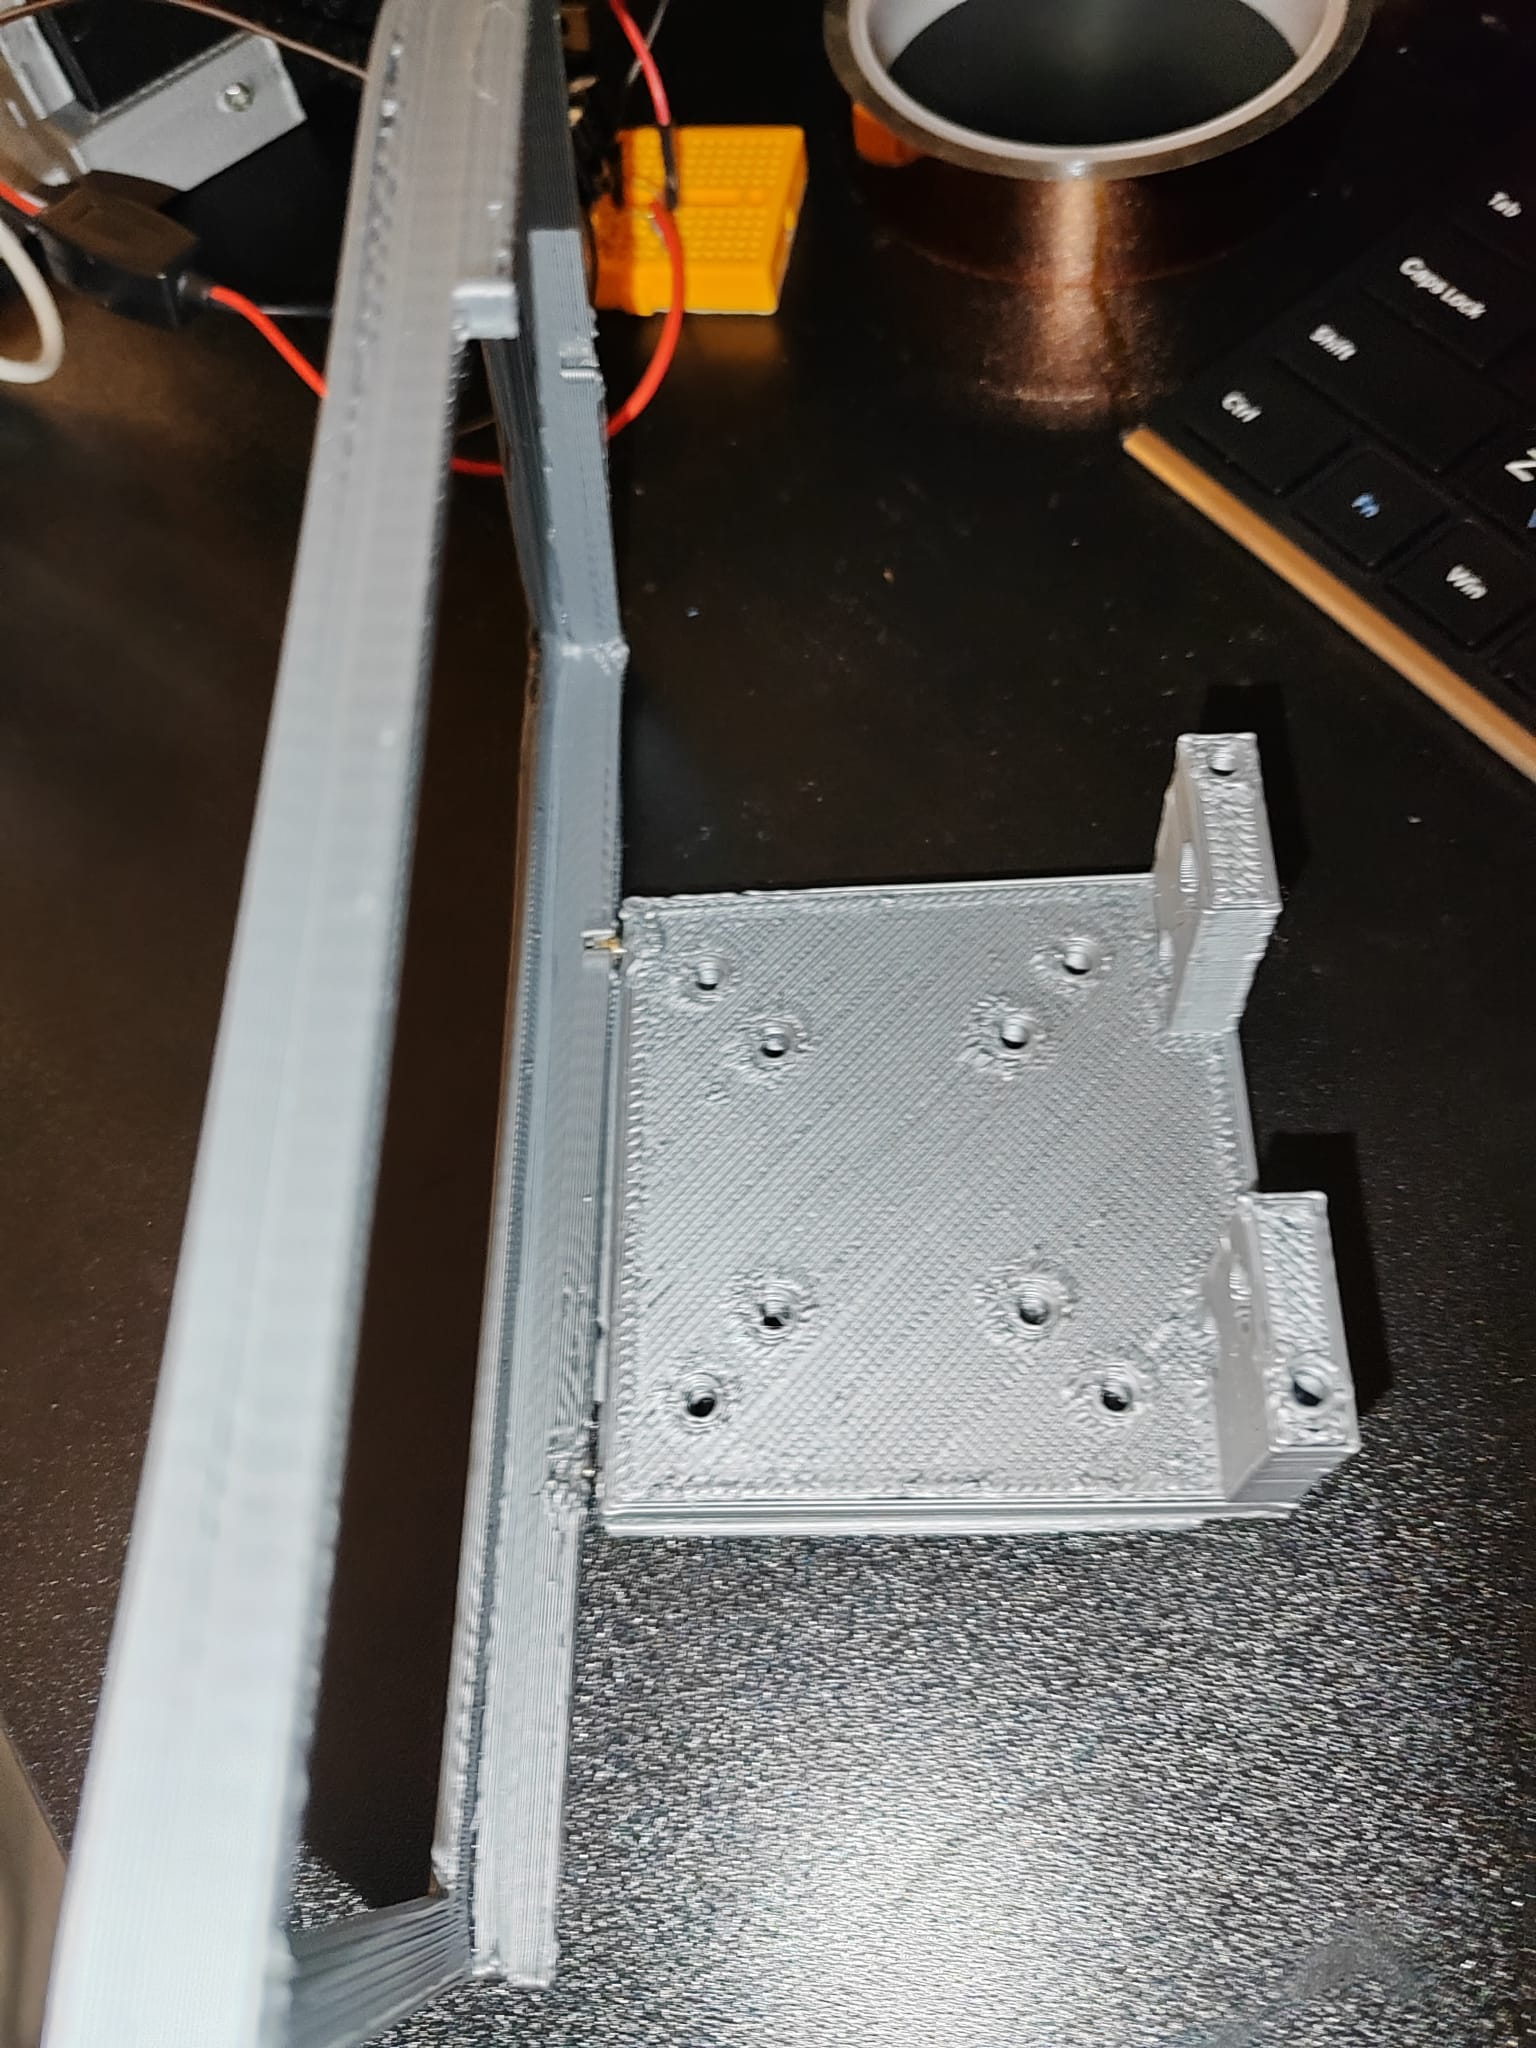
\includegraphics[width=\textwidth]{imgs/design/unbracedscreen.jpeg}
    \caption{Unbraced Screen}
    \label{fig:unbracedscreen}
  \end{minipage}
  \hfill
  \begin{minipage}[t]{0.24\textwidth}
    \centering
    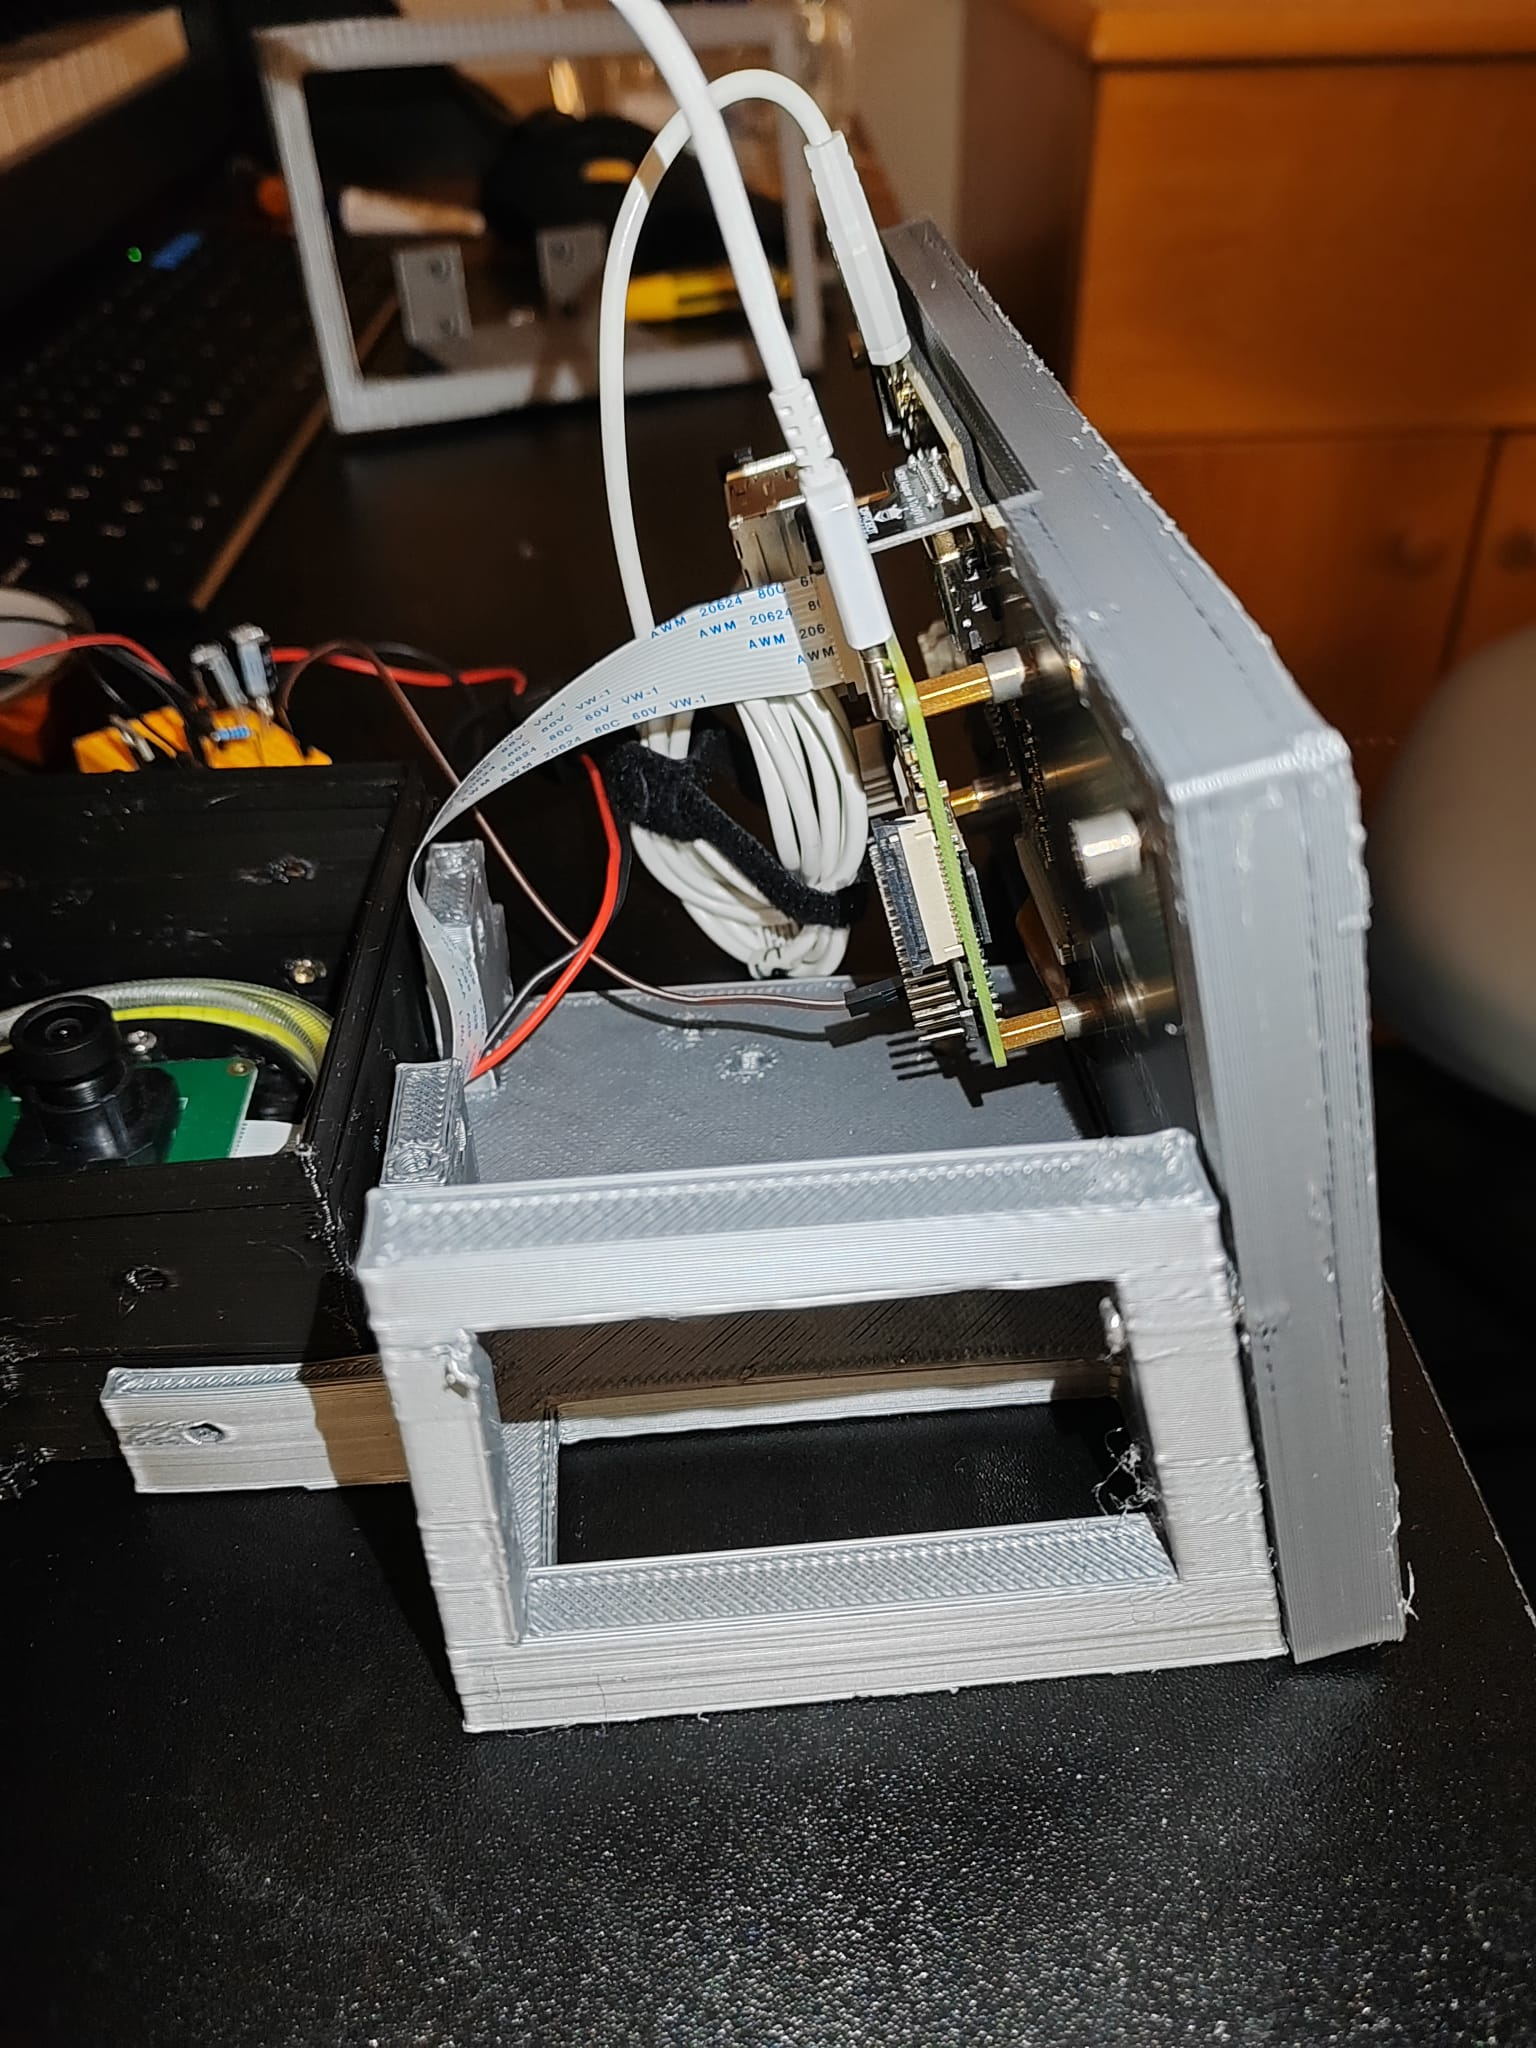
\includegraphics[width=\textwidth]{imgs/design/bracedscreen.jpeg}
    \caption{Braced Screen}
    \label{fig:bracedscreen}
  \end{minipage}
  \hfill
  \begin{minipage}[t]{0.24\textwidth}
    \centering
    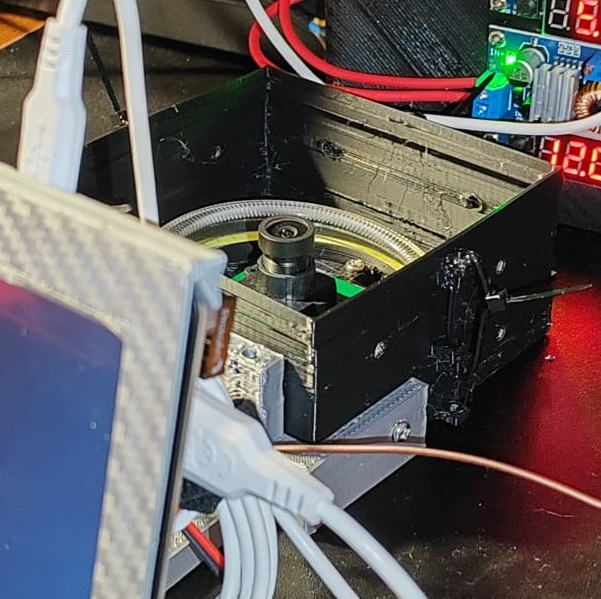
\includegraphics[width=\textwidth]{imgs/design/shortcamera.jpeg}
    \caption{Short Camera Housing}
    \label{fig:shortcamera}
  \end{minipage}
  \hfill
  \begin{minipage}[t]{0.24\textwidth}
    \centering
    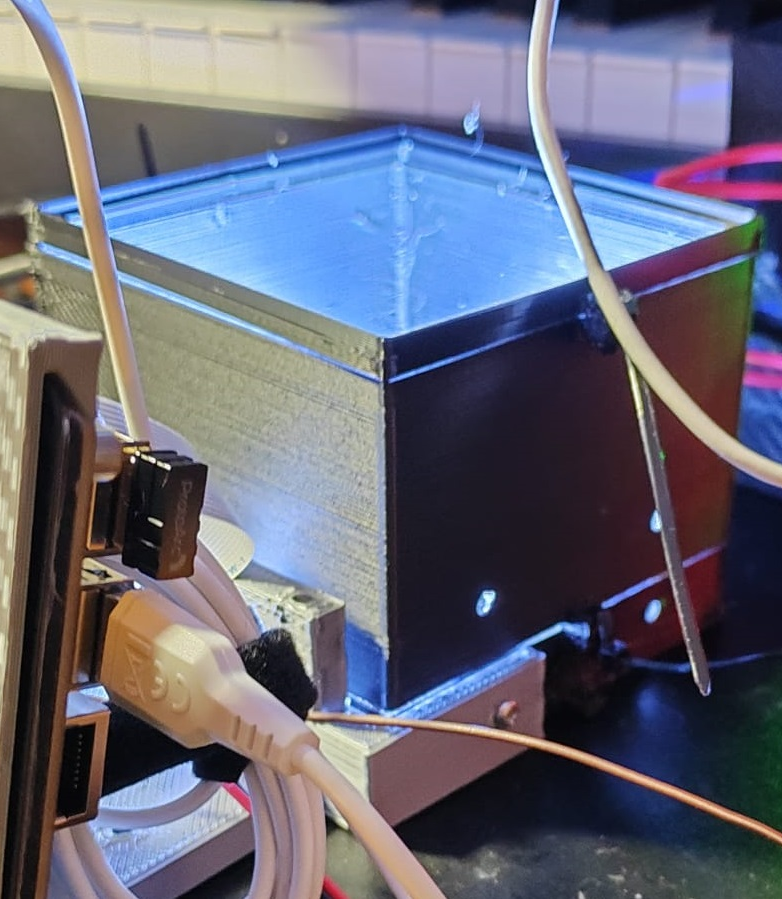
\includegraphics[width=\textwidth]{imgs/design/tallcamera.jpeg}
    \caption{Optimal Camera Housing}
    \label{fig:tallcamera}
  \end{minipage}
\end{figure*}

However, in the end none of these could be considered because of the electronics design problem discussed in the following section.
\noindent
\textbf{Electronics Design Problems} \\
Attempting to dim the LED Ring resulted in very spoaradic flickering, and it did not react with changes to the frequency of the PWM signal despite the MOSFET control circuit shown in Figure \ref*{fig:wiringschematic}.
Originally, I considered that the issue was with the MOSFET as I had initially used a MOSFET with a higher gate threshold voltage, and so I replaced it with a MOSFET with a lower gate threshold voltage.
However, this did not solve the issue, and I also attempted to add a capacitor in parallel to the LED Ring to buffer the current, but to no avail.
The LED Ring seemed to be a simple ring of LEDs, with no additional circuitry, so it was not clear it was not dimmable.
My supervisor Dr. Stott was also unsure as to why it was not dimmable, and proposed a different circuit with an inductor and diode but this requires
a much higher switching frequency than the Pi's PWM signal can provide, and so it was not viable. 

For these reasons, and after reviewing literature as dicussed in Section \ref*{sec:background}, I decided to redesign the camera mount to be down-facing (as I may require a conveyer belt in the future),
and replace the LED Ring with a WS2812B LED strip, as these are known to be dimmable (as I have personal experience with them). They are also addressable, however this is not a feature that I will be using in this stage of the project.
